% questions.tex —— 1993 年·上海卷 · 题目内容片段（无答案）
% 由 tools/generate_projects.py 依来源总账自 1993/1993_上海_试题.md 生成，勿手改（改源 MD 后重跑）


\begin{gktip}
卷面抬头：1993 年全国普通高等学校招生统一考试　上海　数学试题

卷首「考生注意」：这份试卷共有 26 道试题，满分 150 分。
\end{gktip}

\gkpart{一、填空题（本大题满分 30 分）本大题共有 10 题，只要求直接填写结果，每个空格填对得 3 分，否则一律得零分。}

\begin{question}
\gkti{1}函数 $y=x^2-2x+3$ 的最小值是 \gkblank{}。

\end{question}
\begin{question}
\gkti{2}函数 $y=\cos^2(\omega x)$（$\omega>0$）的最小正周期是 \gkblank{}。

\end{question}
\begin{question}
\gkti{3}设 $z=\cos\dfrac{7\pi}{5}+i\sin\dfrac{7\pi}{5}$，$i$ 是虚数单位，则 $\bar z$ 的辐角主值是 \gkblank{}。

\end{question}
\begin{question}
\gkti{4}1 名老师和 4 名获奖同学排成一排照相留念，若老师不排在两端，则共有不同排法 \gkblank{} 种（结果用数值表示）。

\end{question}
\begin{question}
\gkti{5}函数 $y=\arccos x$（$-1\le x\le 0$）的反函数是 \gkblank{}。

\end{question}
\begin{question}
\gkti{6}$P$ 点分 $\overline{AB}$ 所成的比是 $-3$，则 $B$ 点分 $\overline{AP}$ 所成的比是 \gkblank{}。

\end{question}
\begin{question}
\gkti{7}已知圆台的上、下底面半径分别是 $10\,\mathrm{cm}$ 和 $20\,\mathrm{cm}$，它的侧面展开后所得扇环的圆心角是 $180^\circ$，那么圆台的侧面积是 \gkblank{} $\mathrm{cm}^2$（结果中保留 $\pi$）。

\end{question}
\begin{question}
\gkti{8}已知等比数列 $\{a_n\}$（$a_n\in\mathbb{R}$），$a_1+a_2=9$，$a_1\cdot a_2\cdot a_3=27$，且 $S_n=a_1+a_2+\cdots+a_n$（$n=1,2,\ldots$），则 $\lim\limits_{n\to\infty}S_n=$ \gkblank{}。

\end{question}
\begin{question}
\gkti{9}在极坐标系中，过点 $M\left(2,\dfrac{\pi}{2}\right)$ 且平行于极轴的直线的极坐标方程是 \gkblank{}。

\Needspace{0.4\textheight}
\end{question}
\begin{question}
\gkti{10}如图，正方体 $ABCD-A_1B_1C_1D_1$ 中，过顶点 $B$、$D$、$C_1$ 作截面，则二面角 $B\text{-}DC_1\text{-}C$ 的大小是 \gkblank{}（用反三角函数表示）。
\nopagebreak[4]
\begin{center}% 依固定扫描页重绘；仅示意正方体的拓扑、顶点标号与过 B、D、C_1 的截面，不按比例。
% 投影坐标只为作图，不表示题设给出坐标或边长。下底面为 ABCD，上底面为 A_1B_1C_1D_1。
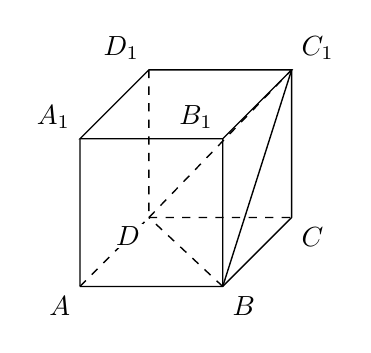
\begin{tikzpicture}[line width=.5pt,scale=1.25]
  \coordinate (A1) at (0,1.7);
  \coordinate (B1) at (1.45,1.7);
  \coordinate (C1) at (2.15,2.4);
  \coordinate (D1) at (.7,2.4);
  \coordinate (A) at (0,.2);
  \coordinate (B) at (1.45,.2);
  \coordinate (C) at (2.15,.9);
  \coordinate (D) at (.7,.9);
  % 上底面、可见外棱与隐藏外棱。
  \draw (A1)--(B1)--(C1)--(D1)--cycle;
  \draw (A1)--(A) (B1)--(B) (C1)--(C) (A)--(B)--(C);
  \draw[dashed] (D1)--(D) (A)--(D) (D)--(C);
  % 截面 BDC_1：BD 位于下底面、DC_1 位于背面，按投影用虚线表示。
  \draw (B)--(C1);
  \draw[dashed] (B)--(D) (D)--(C1);
  \node[above left] at (A1) {$A_1$};
  \node[above left] at (B1) {$B_1$};
  \node[above right] at (C1) {$C_1$};
  \node[above left] at (D1) {$D_1$};
  \node[below left] at (A) {$A$};
  \node[below right] at (B) {$B$};
  \node[below right] at (C) {$C$};
  \node[fill=white,inner sep=1pt,below left=2pt] at (D) {$D$};
\end{tikzpicture}
\end{center}
\nopagebreak[4]
\end{question}
\gkpart{二、选择题（本大题满分 30 分）本大题共有 10 题，每题都给出代号为 A、B、C、D 的四个结论，其中有且只有一个结论是正确的，必须把正确结论的代号写在题后的圆括号内，选对得 3 分，不选、选错或者选出的代号超过一个（不论是否都写在圆括号内），一律得零分。}

\Needspace{0.4\textheight}
\begin{question}
\gkti{11}函数 $y=x+a$ 与 $y=\log_a x$ 的图象可能是（　）。

（A）图 A；（B）图 B；（C）图 C；（D）图 D。
\nopagebreak[4]
\begin{center}% 依固定扫描页重绘；四个面板只示意直线 y=x+a 的截距位置与曲线 y=log_a x 的增减方向，不按比例。
% 只有 (C) 用同一个 0<a<1 同时满足两函数的图象特征。
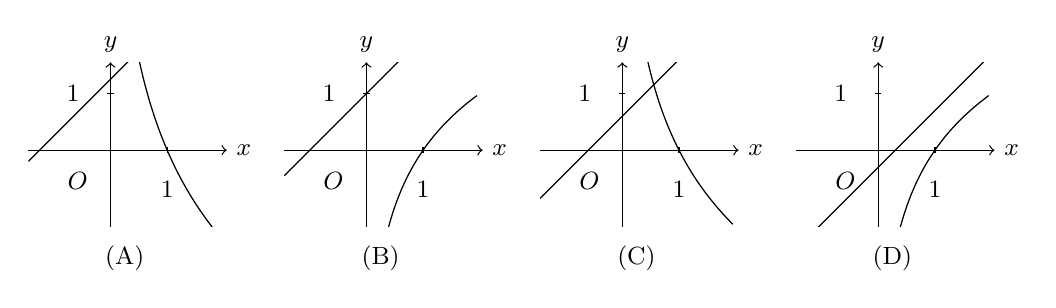
\begin{tikzpicture}[line width=.45pt,x=.72cm,y=.72cm,font=\small]
  \foreach \panel/\shift/\linea/\loga in {A/0/1.25/.65,B/3.25/1/2,C/6.5/.6/.6,D/9.75/-.3/2}{
    \begin{scope}[xshift=\shift cm]
      \begin{scope}
        \clip (-1.45,-1.35) rectangle (2.05,1.55);
        \draw[domain=.34:1.95,samples=70,smooth] plot (\x,{ln(\x)/ln(\loga)});
        \draw[domain=-1.45:2.05,samples=2] plot (\x,{\x+\linea});
      \end{scope}
      \draw[->] (-1.45,0)--(2.05,0) node[right] {$x$};
      \draw[->] (0,-1.35)--(0,1.55) node[above] {$y$};
      \draw (-.055,1)--(.055,1);
      \node[left=10pt,inner sep=1pt] at (0,1) {$1$};
      \draw (1,-.055)--(1,.055);
      \node[below=10pt,inner sep=1pt] at (1,0) {$1$};
      \node[below left=7pt,inner sep=1pt] at (0,0) {$O$};
      \node at (.25,-1.9) {(\panel)};
    \end{scope}
  }
\end{tikzpicture}
\end{center}
\nopagebreak[4]
\end{question}
\begin{question}
\gkti{12}$(x-1)^9$ 按 $x$ 降幂排列的展开式中，系数最大的项是（　）。

（A）第 4 项和第 5 项；（B）第 5 项；（C）第 5 项和第 6 项；（D）第 6 项。

\end{question}
\begin{question}
\gkti{13}在区间 $(0,+\infty)$ 上为增函数的是（　）。

（A）$y=\operatorname{arcctg}x$；（B）$y=\log_{1/2}x$；（C）$y=-2^x$；（D）$y=x^{1/3}$。

\end{question}
\begin{question}
\gkti{14}下列不等式中正确的是（　）。

（A）$\arcsin\left(-\dfrac14\right)<\arcsin\left(-\dfrac13\right)$；

（B）$\arccos\left(-\dfrac14\right)<\arccos\dfrac13$；

（C）$\operatorname{arctg}\dfrac14<\arcsin\dfrac14$；

（D）$\operatorname{arcctg}\dfrac13<\operatorname{arctg}\dfrac13$。

\end{question}
\begin{question}
\gkti{15}动点 $P$ 到直线 $x+4=0$ 的距离减去它到点 $M(2,0)$ 的距离之差等于 2，则点 $P$ 的轨迹是（　）。

（A）直线；（B）椭圆；（C）双曲线；（D）抛物线。

\end{question}
\begin{question}
\gkti{16}设有三个命题：

甲、底面是平行四边形的四棱柱是平行六面体；

乙、底面是矩形的平行六面体是长方体；

丙、直四棱柱是直平行六面体。

以上命题中真命题的个数是（　）。

（A）0；（B）1；（C）2；（D）3。

\end{question}
\begin{question}
\gkti{17}在直角坐标系中平移坐标轴，把原点 $O(0,0)$ 移到 $O'(2,-5)$，点 $A$ 在新坐标系中的坐标为 $(-3,7)$，则点 $A$ 在原坐标系中的坐标是（　）。

（A）$(-1,2)$；（B）$(1,-2)$；（C）$(-5,12)$；（D）$(5,-12)$。

\end{question}
\begin{question}
\gkti{18}设 $a$、$b$ 是两条异面直线。在下列命题中正确的是（　）。

（A）有且仅有一条直线与 $a$、$b$ 都垂直；

（B）有一平面与 $a$、$b$ 都垂直；

（C）过直线 $a$ 有且仅有一平面与 $b$ 平行；

（D）过空间中任一点必可作一条直线与 $a$、$b$ 都相交。

\end{question}
\begin{question}
\gkti{19}函数 $y=\cos\left(2x+\dfrac{\pi}{2}\right)$ 的图象的一条对称轴方程是（　）。

（A）$x=-\dfrac{\pi}{2}$；（B）$x=-\dfrac{\pi}{4}$；（C）$x=\dfrac{\pi}{8}$；（D）$x=\pi$。

\end{question}
\begin{question}
\gkti{20}“$a+b>2c$”的一个充分条件是（　）。

（A）$a>c$ 或 $b>c$；（B）$a>c$ 且 $b<c$；（C）$a>c$ 且 $b>c$；（D）$a>c$ 或 $b<c$。

\end{question}
\gkpart{三、（本大题满分 36 分）本大题共有 3 题，解下列各题必须写出必要的步骤。}

\begin{question}
\gkti{21}（本题满分 12 分）

已知角 $\alpha$ 的顶点与直角坐标系的原点重合，始边在 $x$ 轴的正半轴上，终边经过点 $P(-1,2)$，求 $\sin\left(2\alpha+\frac{2\pi}{3}\right)$ 的值。

\end{question}
\begin{question}
\gkti{22}（本题满分 12 分）

已知 $z=\dfrac{a-i}{1-i}$，其中 $i$ 为虚数单位，$a>0$，复数 $w=z(z+i)$ 的虚部减去它的实部所得的差等于 $\dfrac32$，求复数 $w$ 的模。

\end{question}
\begin{question}
\gkti{23}（本题满分 12 分）

抛物线 $y=-\dfrac{x^2}{2}$ 与过点 $M(0,-1)$ 的直线 $l$ 相交于 $A$、$B$ 两点，$O$ 为坐标原点。若直线 $OA$ 与 $OB$ 的斜率之和为 1，求直线 $l$ 的方程。

\end{question}
\gkpart{四、（本大题满分 54 分）本大题共有 3 题，解下列各题必须写出必要的步骤。}

\Needspace{0.4\textheight}
\begin{question}
\gkti{24}（本题满分 16 分）本题共有 3 小题，第 1 小题满分 5 分，第 2 小题满分 5 分，第 3 小题满分 6 分。

如图，已知二面角 $\alpha\text{-}PQ\text{-}\beta$ 为 $60^\circ$，点 $A$ 和点 $B$ 分别在平面 $\alpha$ 和平面 $\beta$ 上，点 $C$ 在棱 $PQ$ 上，$\angle ACP=\angle BCP=30^\circ$，$CA=CB=a$。

（1）求证 $AB\perp PQ$；

（2）求点 $B$ 到平面 $\alpha$ 的距离；

（3）设 $R$ 是线段 $OA$ 上的一点，直线 $BR$ 与平面 $\alpha$ 所成角的大小为 $45^\circ$，求线段 $CR$ 的长度。
\nopagebreak[4]
\begin{center}% 依固定扫描页重绘；两平面以平行四边形示意，交棱为 PQ，A 在平面 α 内，B 在平面 β 内，C 在 PQ 上。
% 面片与投影仅为拓扑示意，不按比例；不编码题面未给出的长度、角度、垂足或点 O 的定义。
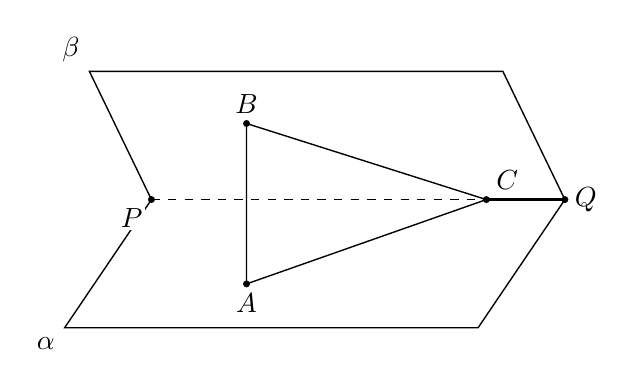
\begin{tikzpicture}[line width=.5pt,scale=1.05]
  \coordinate (P) at (0,0);
  \coordinate (Q) at (5,0);
  \coordinate (BtL) at (-.75,1.55);
  \coordinate (BtR) at (4.25,1.55);
  \coordinate (AlL) at (-1.05,-1.55);
  \coordinate (AlR) at (3.95,-1.55);
  \coordinate (A) at (1.15,-1.02);
  \coordinate (B) at (1.15,.92);
  \coordinate (C) at (4.05,0);
  % 两个平面以平行四边形作投影边界，共用棱 PQ。
  \draw (P)--(BtL)--(BtR)--(Q);
  \draw (P)--(AlL)--(AlR)--(Q);
  \draw[dashed] (P)--(C);
  \draw[thick] (C)--(Q);
  % 原图中的三角形 ABC 与交棱关系。
  \draw (A)--(B)--(C)--cycle;
  \fill (P) circle (1.2pt) (Q) circle (1.2pt) (A) circle (1.2pt)
    (B) circle (1.2pt) (C) circle (1.2pt);
  \node[fill=white,inner sep=1pt,below left=2pt] at (P) {$P$};
  \node[right] at (Q) {$Q$};
  \node[below] at (A) {$A$};
  \node[above] at (B) {$B$};
  \node[above right] at (C) {$C$};
  \node[above left] at (BtL) {$\beta$};
  \node[below left] at (AlL) {$\alpha$};
\end{tikzpicture}
\end{center}
\nopagebreak[4]
\end{question}
\begin{question}
\gkti{25}（本题满分 18 分）本题共有 3 小题，第 1 小题满分 5 分，第 2 小题满分 5 分，第 3 小题满分 8 分。

设数列 $\{a_n\}$ 的前 $n$ 项和 $S_n=na+n(n-1)b$（$n=1,2,\ldots$），$a$、$b$ 是常数且 $b\ne 0$。

（1）证明 $\{a_n\}$ 是等差数列；

（2）证明以 $\left(a_n,\dfrac{S_n}{n}-1\right)$ 为坐标的点 $P_n$（$n=1,2,\ldots$）都落在同一条直线上，并写出此直线的方程；

（3）设 $a=1$，$b=\dfrac12$，$C$ 是以 $(r,r)$ 为圆心、$r$ 为半径的圆（$r>0$）。求使得点 $P_1$、$P_2$、$P_3$ 都落在圆 $C$ 外时，$r$ 的取值范围。

\Needspace{0.4\textheight}
\end{question}
\begin{question}
\gkti{26}（本题满分 20 分）本题共有 3 小题，第 1 小题满分 6 分，第 2 小题满分 8 分，第 3 小题满分 6 分。

如图，$P$ 为椭圆 $\dfrac{x^2}{a^2}+y^2=1$ 上的一个动点，它与长轴端点不重合，$a\ge\sqrt2$，点 $F_1$ 和 $F_2$ 分别是双曲线 $\dfrac{x^2}{a^2}-y^2=1$ 的左焦点和右焦点，$\varphi=\angle F_1PF_2$。

（1）求 $\operatorname{tg}\varphi$ 的表达式（用 $a$ 及描述点 $P$ 位置的一个变量来表示）；

（2）当 $a$ 固定时，求 $\varphi$ 的最小值 $\varphi_0$；

（3）当 $a$ 在区间 $[\sqrt2,\sqrt3]$ 上变化时，求 $\varphi_0$ 的取值范围。
\nopagebreak[4]
\begin{center}% 依固定扫描页重绘；椭圆 x^2/a^2+y^2=1、双曲线 x^2/a^2-y^2=1 及其焦点、动点 P 与角 φ 的拓扑示意，不按比例。
% 取 a=1.6 仅用于示意绘图，满足 a>=sqrt(2)；不把该数值加入题面条件。
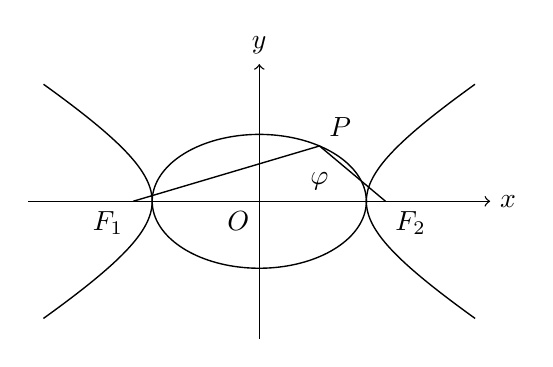
\begin{tikzpicture}[line width=.5pt,x=.85cm,y=.85cm]
  \pgfmathsetmacro{\a}{1.6}
  \pgfmathsetmacro{\f}{sqrt(\a*\a+1)}
  \pgfmathsetmacro{\px}{.9}
  \pgfmathsetmacro{\py}{sqrt(1-(\px/\a)*(\px/\a))}
  \coordinate (O) at (0,0);
  \coordinate (F1) at (-\f,0);
  \coordinate (F2) at (\f,0);
  \coordinate (A1) at (-\a,0);
  \coordinate (A2) at (\a,0);
  \coordinate (P) at (\px,\py);
  \coordinate (H) at (\px,0);
  \draw[->] (-3.45,0)--(3.45,0) node[right] {$x$};
  \draw[->] (0,-2.05)--(0,2.05) node[above] {$y$};
  \draw[domain=0:360,samples=150,smooth]
    plot ({\a*cos(\x)},{sin(\x)});
  \draw[domain=-1.75:1.75,samples=100,smooth]
    plot ({\a*sqrt(1+\x*\x)},\x);
  \draw[domain=-1.75:1.75,samples=100,smooth]
    plot ({-\a*sqrt(1+\x*\x)},\x);
  \draw (F1)--(P)--(F2);
  \node[below left] at (O) {$O$};
  \node[below left] at (F1) {$F_1$};
  \node[below right] at (F2) {$F_2$};
  \node[above right] at (P) {$P$};
  \node[below=6pt] at (P) {$\varphi$};
\end{tikzpicture}
\end{center}
\nopagebreak[4]

\end{question}